%\documentclass[Proof]{elex}
\documentclass{elex}

\usepackage[dvips]{graphicx}

\vol{*}
\no{*}

\title{Instructions/template for\\
preparing your ELEX\\
manuscript (As of March 1, 2010)}

\author{Hiroshi Toshiyoshi,$^{1}$ Kazukiyo Joshin,$^{2}$ and Takuji Takahashi$^{1}$}

\affiliate{
$^{1}$ Institute of Industrial Science, University of Tokyo\\
4-6-1 Komaba, Meguro-ku, Tokyo 153-8505, Japan \\
%
$^{2}$ Photo Electronics Lab, Fujitsu Laboratories Co. \\
10-1 Wakamiya, Morinosato, Atsugi, Kanagawa 243-0197, Japan
}

\email{hiro@iis.u-tokyo.ac.jp}

\received{2003}{7}{00}
\accepted{2003}{7}{00}


\setcounter{page}{1}

\begin{document}

\maketitle 

\begin{abstract} 

Use this instruction file as a template for preparing your ELEX articles with LaTeX.  It is essential to adhere to this template because your manuscripts are printed as submitted with minimal editing/formatting by publisher.  Do not modify any formats or styles.  Main text is limited to 1,500 words, and abstract is about 100 words. You may include total maximum three display items (Figures and Tables) in principle but do not exceed 2 MB after converting to PDF.  Use latest Adobe Acrobat to attach movie pictures in your PDF version of manuscript.  Visit
http://www.elex.ieice.org for the latest version of ELEX template.
\end{abstract}

\begin{keywords}
ELEX, template, elex.cls, up to six words
\end{keywords}

\begin{classification}
XYZ (choose one from Table II)
\end{classification}


\begin{thebibliography}{99}

\bibitem{journal paper} A. B. Author1, C. D. Author2, and E. F. Author3, "Title of journal paper with a comma inside the quotation marks like this," {\it Journal Title in Italic} vol. 12, no. 3, pp. 456-789, month, year.

\bibitem{chapter} A. B. Chapter-Writer, "Title of quoted chapter" in {\it Book Title in Italic without Quotation Marks}, ed. C. D. Editor, pp. 123-456, Publisher Name, City, year.

\bibitem{book} A. B. Book-Author, Book {\it Title in Italic without Quotation Marks}, Publisher Name, City, year.


\bibitem{proceeding paper} A. B. Author1, C. D. Author2, and E. F. Author3, "Title of paper in proceeding," Proc. 12th Conf. Name, City, Country, paper ID, pp. 123-456, month, year.


\bibitem{web link} Visit \underline{http://www.elex.ieice.org} for latest version of this template.


\end{thebibliography}


\section{Introduction}

This template provides formats and styles for ELEX manuscript. It is essential to adhere to this template because your manuscript will be published "{\it as is}" with minimal copy-editing by the publisher.  Do not modify formats (font, font size, paper size, printing area, line space, etc).  {\it Keep one copy of this template untouched for your reference and prepare your manuscript on another copy.}


\section{Software and article charge}


Microsoft Word and LaTeX compatible files are officially acceptable for ELEX submission. This template file is designed for MS Word.  LaTeX style files can be found elsewhere\cite{web link}.  Article charge is JPY~31,500 for a manuscript using MS Word template and JPY~21,000 for a manuscript using LaTeX style file. Including movie picture(s) costs extra JPY 3,150 per movie file.


\section{Manuscript length} 

Papers do not usually exceed six (6) pages of an A4-sized PDF file.  The first page contains paper title, author list, affiliation(s), 100-word-abstract, keywords, and references.  The main body of the text is limited to approximately 1,500 words.  Manuscripts are allowed to have up to three (3) display items (Figures and/or Tables) with brief captions in principle as long as the final PDF file size would not exceed 2 MB.  Including multimedia files (movie graphics) in a final PDF file is possible, if any, by using attachment function of Adobe Acrobat.


\section{Typographical style}


Consult with Table~\ref{tab:style} on the detail typographical styles. 


\begin{table}[ht]
\begin{center}
\caption{ELEX typographical style} \label{tab:style}
\begin{small}
\begin{tabular}{lcl}
\hline
Article title & \quad &  Arial 26pt Bold Green\\
\hline
Author Name & \quad & Times New Roman 12pt Bold Black\\
\hline
Author Affiliation & \quad & Times New Roman 10pt Italic Black\\
\hline
Author Address & \quad & Times New Roman 10pt Italic Black\\
\hline
Author Contact E-mail & \quad & Times New Roman 10pt Italic Blue\\
\hline
Section Heading & \quad & Arial 11pt Bold Black\\
(incl. "Abstract" and "Keywords") & & \\
\hline
Abstract Body & \quad & Times New Roman 11pt Black\\
\hline
Reference Body & \quad & Times New Roman 10pt Black\\
\hline
Section Title & \quad & Arial 12pt Bold Black\\
\hline
Text Body & \quad & Times New Roman 11pt Black\\
\hline
Figure \& Table Label in Caption & \quad & Times New Roman 10pt Bold Black\\
\hline
Figure \& Table Caption Body & \quad & Times New Roman 10pt Black\\
\hline
Acknowledgement Body & \quad & Times New Roman 11pt Black\\
\hline
\end{tabular}
\end{small}
\end{center}
\end{table}


\subsection{Title}

Title should start flush left.  Only the first letter in the title is capitalized (this is true to section titles and figure captions) Avoid including abbreviations unless definitely needed.


\subsection{Author name and affiliation}

Author names should start flush left.  Spell out both first and last names but initial middle name. Use one blank line between authors from different affiliations.


\subsection{Abstract}

The abstract should be complete sentence(s) that is limited to approximately 100 words.  It should be a concise summary of the paper that clearly conveys the problem, the methods, and the conclusions to readers.  It also should include appropriate keywords for the convenience of computer search.  Do not include reference numbers.

\subsection{Keywords}

Maximum six (6) keywords are listed.  Carefully choose appropriate keywords for your paper being correctly spotted by computerized search.


\subsection{Classification}

Category index in the classification is used by the ELEX Editorial Office when directing your manuscript to corresponding Associate Editor. Furthermore it is displayed in ELEX website and in archives for readers' convenience. Choose most relevant category from Table~\ref{tab:classification}. The Editorial Committee may change the subject index that authors select, if the Editorial Committee judges that the authors' selection is not the best.  Note that the index might be changed without notification. 




\begin{table}[ht]
\begin{center}
\caption{ELEX category classification (As of October 1, 2008)} \label{tab:classification}
\begin{small}
\begin{tabular}{l}
\hline
Optoelectronics, Lasers and quantum electronics, Ultrafast optics,  \\
Silicon photonics, Planar lightwave circuits \\
\hline
Fiber optics, Microwave photonics, Optical interconnection,  \\
Photonic signal processing, Photonic integration and systems \\
\hline
Electromagnetic theory \\
\hline
Microwave and millimeter wave devices, circuits, and systems \\
\hline
Electron devices, circuits, and systems \\
\hline
Integrated circuits \\
\hline
Micro- or nano-electromechanical systems \\
\hline
Storage technology \\
\hline
Superconducting electronics \\
\hline
Electronic materials, semiconductor materials \\
\hline
Electronic displays \\
\hline
Organic molecular electronics, Polymer optical circuits \\
\hline
Ultrasonic electronics \\
\hline
Electron tubes, vacuum and beam technology \\
\hline
Electronic instrumentation and control \\
\hline
Wireless circuits and devices \\
\hline
Electromagnetic compatibility (EMC) \\
\hline
Fiber-optic communication \\
\hline
Optical fiber \\
\hline
Science and engineering for electronics \\
\hline
\end{tabular}
\end{small}
\end{center}
\end{table}


\subsection{Main text and headings}

Single column format is applied throughout the manuscript. The first line of the first paragraph of each section start flush left.  Section headings are numbered consecutively in Arabic numbers.  Subsection headings are numbered in Arabic numbers to the right of the decimal point (like this 4.5).

\subsection{Equations}

Equations are centered with the equation number (in Arabic) appearing at the right-hand margin, in parenthesis:
\begin{equation}
T_{\mbox{M}}^{\phi} = 2 \times \frac{G w t^3}{3 l} \phi \left( 1 - \frac{192}{\pi^5} {\frac{t}{w}} \tanh \frac{\pi w}{2 t} \right).
\end{equation}
\noindent
Long equations can be folded in several lines but avoid leading to
misinterpretation.  Equations are referenced in the main text as Eq. (1).


\subsection{References}

References should appear on the first page of the paper, in the order in which they are referred in the main text.  See the example in this template for different styles for citing a journal paper, a whole book, a contributed chapter in a book and a proceeding paper.  WWW links can be placed as a reference.  It is authorsf responsibility to provide correct information of references. Use a pair of square bracket to cite reference like this [2].  Multiple references can be cited by using a hyphen like this [2-5].


\subsection{Acknowledgements}

Acknowledgements, if any, can be placed at the end of the manuscript.


\section{Display items (figures, tables, and movies)}

You may include total maximum three (3) pieces of display items in principle in a final PDF version of your manuscript but do not exceed 2 MB file size.

\subsection{Figures}

Figures should be placed in the document.  Do not submit figures in separate files.  Use LaTeX environment "\\begin{figure}" to place frames for figures. Place your figure as close to as the main text where it is referred.  Figure position in published paper may differ from that in your original file, when publisher adjusts the final format. Figures are numbered in Arabic numerals. Figures are referred as Fig.~\ref{fig:scanner} even at the beginning of a sentence. Figure captions are placed under corresponding figures.


\begin{figure}[htb]
\begin{center}
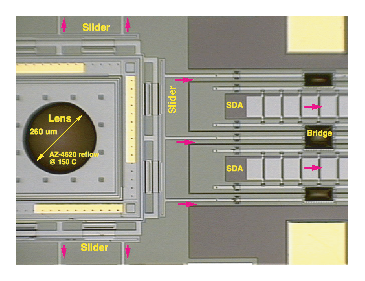
\includegraphics[width=8cm]{figures/lens_scanner.eps}
\end{center}
\caption{Include all graphics in the manuscript file.  Do not submit figures in
separate files.}
\label{fig:scanner}
\end{figure}



\subsection{Tables}

Tables are placed in the document in the same manner as figures.  Tables are referred in Roman numbers such as Table~\ref{tab:style}, without abbreviating to Tab.~\ref{tab:style}.  Table captions are placed above the corresponding tables.



\subsection{Movie files}

It is one of the ELEX features that author could include movie files (mov or mpg) in their final PDF manuscript.  Use file attachment tool of Adobe Acrobat (not Acrobat Reader):
\begin{enumerate}
\item Select the file attachment tool 
\includegraphics[width=5mm]{figures/pin.eps}.
\item Select the location where the movie file is placed (in the figure box).
\item Select the movie file from a dialog box.
\item In the comment properties, set the desired options, if needed.
\item Click OK
\end{enumerate}
Movie files are represented by an Adobe Acrobat icon (like this:
\includegraphics[width=8mm]{figures/pin2.eps} ) and activated by clicking on it. To help readers, you need to place a snapshot of the movie file and place it as a figure.  Notice readers that a movie file has been attached (see Fig.~\ref{fig:movie}).

\begin{figure}[htb]
\begin{center}
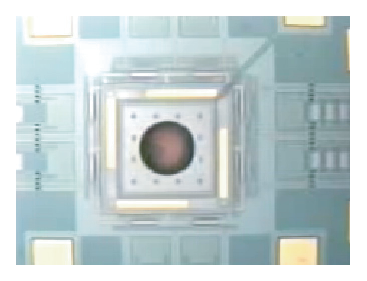
\includegraphics[width=6cm]{figures/snapshot.eps}
\end{center}
\caption{Place a snapshot from the movie file to display for readers.  Movie can be activated by clicking on the icon.  Movie file attached.}
\label{fig:movie}
\end{figure}


\section{Conclusion}

To submit your manuscript to ELEX, visit an IEICE website \\
\verb+(https://review.ieice.org/regist_elex_e.aspx?cmdtype=ELEX)+ \\
to complete a Submission Form and to upload the following items: 
a PDF file for review; an electronic file of manuscript in either 
LaTeX or MS Word; original art work in separate electronic files. 
Art submitted electronically is only acceptable as Encapsulated 
PostScript (.EPS) for graphics and MOV or MPG for movies. 
Self-descriptive file names such as fig1.eps and fig2.mpg are preferred.  
Authors are also requested to select the subject index (code and field) 
best fitting manuscript from the candidates. The index is used by the 
IEICE Publishing Office when directing manuscript to corresponding 
Associate Editor. Furthermore it is displayed in ELEX website and 
in archives for readers' convenience. The Editorial Committee may 
change the subject index that authors select, if the Editorial Committee 
judges that the authors' selection is not the best. Print and fill in 
a downloaded Copyright Transfer and Article Charge Agreement Form, and 
send it to the IEICE Office by postal mail, fax or e-mail. 
If authors fail to print out the Agreement Form provided in manuscript 
submission website, they are advised to use its PDF version 
(http://www.elex.ieice.org/data/copyrightform.pdf). 
The manuscript would be automatically rejected irrespective of 
review results, if the Agreement Form is not received by the 
IEICE Publication Office within three (3) weeks after submission:
\\

\quad \begin{minipage}{11cm}
\noindent
IEICE publishing office\\
The Institute of Electronics, Information and Communication Engineers (IEICE)\\
Kikai-Shinko-Kaikan Bldg.,\\
3-5-8, Shibakoen, Minato-ku, Tokyo, 105-0011 JAPAN\\
Phone: +81-3-3433-6692\\
Fax: +81-3-3433-6616\\
E-mail: ELEX@ieice.org\\
\verb+(https://review.ieice.org/regist_elex_e.aspx?cmdtype=ELEX)+
\end{minipage}

\section*{Acknowledgments}

Your acknowledgements to co-workers and financial sponsors are placed here.

\end{document}
